\documentclass[11pt]{article}

\usepackage[margin=1in]{geometry}
\usepackage{graphicx}
\usepackage{booktabs}
\usepackage{listings}
\usepackage{xcolor}
\usepackage{hyperref}
\usepackage{amsmath}
\usepackage{caption}

\definecolor{codebg}{RGB}{245,247,250}
\lstset{
  basicstyle=\ttfamily\small,
  backgroundcolor=\color{codebg},
  breaklines=true,
  frame=single,
  framerule=0.3pt,
  columns=fullflexible,
  showstringspaces=false,
  xleftmargin=8pt,
  xrightmargin=8pt,
}

\hypersetup{colorlinks=true, linkcolor=black, urlcolor=blue, citecolor=black}

\title{VoiceGuard — Results\\
\large Prosodic Fingerprinting MVP: One-Class SVM Anomaly Detector}
\author{VoiceGuard Project}
\date{\today}

\begin{document}

\maketitle

\begin{abstract}
\noindent
VoiceGuard detects AI-generated voice clones by checking a candidate
clip's prosody — habitual rhythm, pause placement, speaking rate, and
pitch dynamics — against an enrolled speaker's known prosodic habits,
rather than relying on spectral/timbre artifacts. This document reports
the results generated by \texttt{notebooks/results.ipynb}: per-speaker
feature distributions, a leave-one-out self-consistency check of the
One-Class SVM detector, and the status of the full genuine-vs-synthetic
evaluation. \textbf{At the time of writing, no synthetic voice clones
have been collected yet}, so the results here are genuine-data
diagnostics, not the final detection accuracy — that section is
implemented and ready, and will populate automatically once synthetic
clips are added.
\end{abstract}

\tableofcontents

% ------------------------------------------------------------------
\section{Setup}

Two speakers were enrolled, \texttt{krishiv} and \texttt{mary}, each
with 10 genuine voice clips (3--8 seconds, recorded on-device). Each
clip was preprocessed (loudness-normalized, VAD-segmented) and reduced
to an 11-dimensional prosodic feature vector:
\texttt{f0\_mean}, \texttt{f0\_std} (pitch, in semitones relative to
the speaker's own median), \texttt{energy\_mean}, \texttt{energy\_std},
\texttt{speaking\_rate\_mean}, \texttt{pause\_count},
\texttt{pause\_mean\_dur}, \texttt{pause\_var\_dur}, \texttt{npvi}
(rhythm), \texttt{jitter}, and \texttt{shimmer}. The full pipeline is
in \texttt{src/features.py}; see \texttt{docs/HANDOVER.md} for the
complete architecture.

\begin{lstlisting}[language=Python]
import json
import sys
sys.path.insert(0, "../src")
sys.path.insert(0, "../src/models")

import matplotlib.pyplot as plt
import numpy as np
import pandas as pd

from eval import evaluate
from oneclass import leave_one_out_eval

df = pd.read_csv("../data/features/features.csv")
with open("../data/features/f0_reference.json") as f:
    f0_refs = json.load(f)
\end{lstlisting}

% ------------------------------------------------------------------
\section{Feature distributions per speaker}

A sanity check before trusting any detector: do the two speakers'
prosodic fingerprints actually differ? If they didn't, the model would
have nothing to key off.

\begin{table}[h!]
\centering
\caption{Per-speaker mean prosodic feature values (genuine clips, $n=10$ each). Std. deviation in parentheses.}
\label{tab:feature-summary}
\small
\begin{tabular}{lcc}
\toprule
Feature & krishiv & mary \\
\midrule
f0\_mean (semitones) & 1.744 (4.648) & $-$1.241 (4.309) \\
f0\_std (semitones) & 2.185 (0.428) & 2.389 (1.163) \\
energy\_mean & 0.0798 (0.0048) & 0.0779 (0.0027) \\
energy\_std & 0.0594 (0.0064) & 0.0621 (0.0034) \\
speaking\_rate\_mean (onsets/s) & 7.259 (1.001) & 7.238 (1.168) \\
pause\_mean\_dur (s) & 0.0120 & 0.0615 \\
npvi & 108.36 (8.69) & 107.56 (4.24) \\
jitter & 0.0319 (0.0057) & 0.0210 (0.0055) \\
shimmer & 0.1382 (0.0266) & 0.1079 (0.0197) \\
\bottomrule
\end{tabular}
\end{table}

Speaking rate and rhythm (nPVI) are nearly identical between the two
speakers — expected, since both were reading similar sentence types.
\textbf{Jitter and shimmer} (voice-quality measures) show the clearest
separation, with krishiv consistently higher on both.

\begin{lstlisting}[language=Python]
numeric_cols = [
    "f0_mean", "f0_std", "energy_mean", "energy_std", "speaking_rate_mean",
    "pause_count", "pause_mean_dur", "pause_var_dur", "npvi", "jitter", "shimmer",
]
genuine = df[df["label"] == "genuine"]
genuine.groupby("speaker")[numeric_cols].agg(["mean", "std"])
\end{lstlisting}

\begin{figure}[h!]
\centering
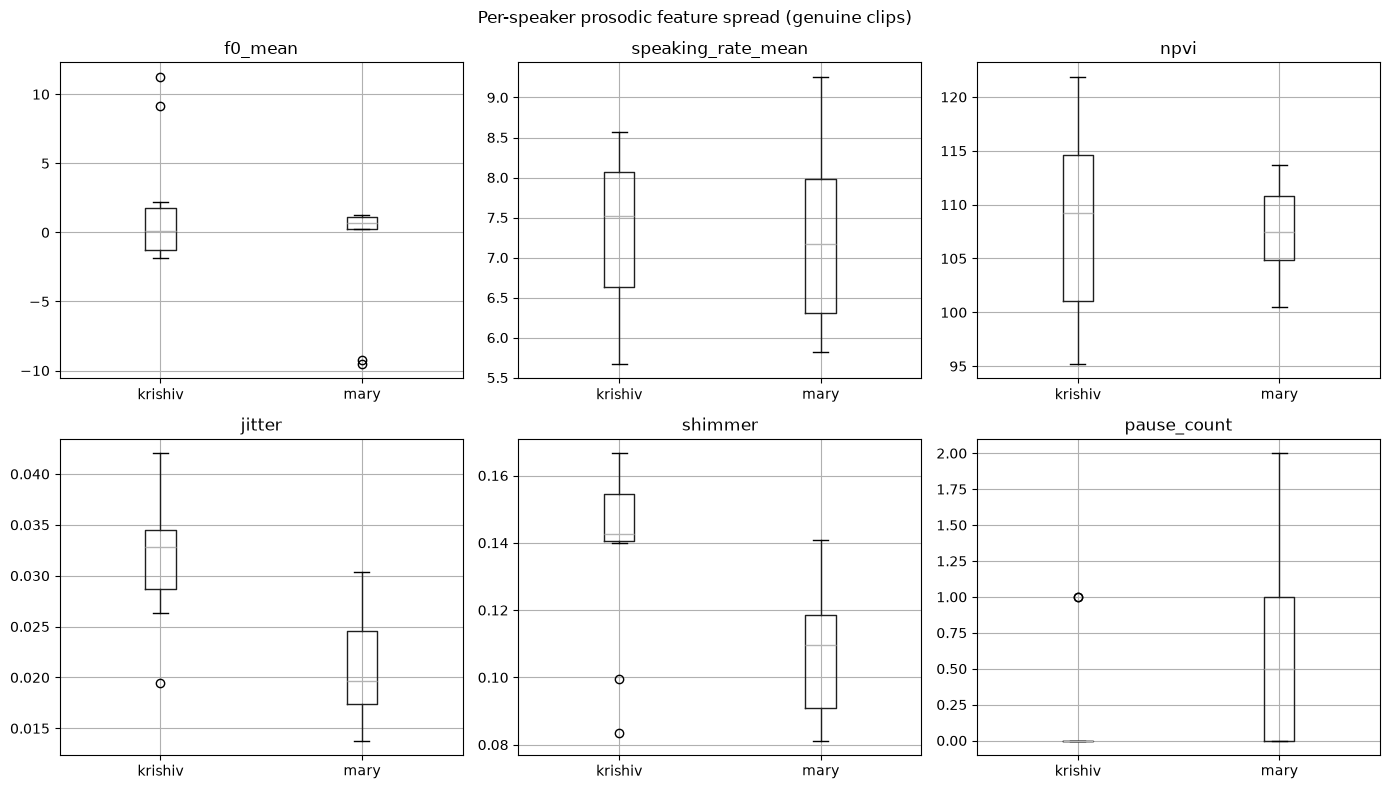
\includegraphics[width=\textwidth]{assets/feature-boxplots.png}
\caption{Per-speaker spread of six representative prosodic features across
their 10 genuine clips.}
\label{fig:boxplots}
\end{figure}

\begin{lstlisting}[language=Python]
fig, axes = plt.subplots(2, 3, figsize=(14, 8))
plot_cols = ["f0_mean", "speaking_rate_mean", "npvi", "jitter", "shimmer", "pause_count"]
for ax, col in zip(axes.flat, plot_cols):
    genuine.boxplot(column=col, by="speaker", ax=ax)
    ax.set_title(col)
    ax.set_xlabel("")
plt.suptitle("Per-speaker prosodic feature spread (genuine clips)")
plt.tight_layout()
plt.show()
\end{lstlisting}

% ------------------------------------------------------------------
\section{Detector: leave-one-out self-consistency}

No synthetic clips exist yet, so this cannot measure
genuine-vs-synthetic discrimination — the detector's actual purpose.
What it \emph{can} check: with each speaker's genuine clip held out in
turn, does their own One-Class SVM (trained on the other 9) still
accept it as genuine?

This is a \textbf{noisy, small-sample diagnostic}, not a target to
hyperparameter-tune against. The linear kernel was chosen over the
default RBF kernel specifically because RBF badly overfits at this
sample size (0--20\% self-acceptance vs. 50--60\% for linear) — see
Section~\ref{sec:kernel} and \texttt{CLAUDE.md} for the full
investigation.

\begin{lstlisting}[language=Python]
for speaker, group in genuine.groupby("speaker"):
    acc, preds = leave_one_out_eval(speaker, group, f0_refs[speaker])
    y_true = [1] * len(preds)
    y_score = [1.0 if p == "genuine" else -1.0 for p in preds]
    metrics = evaluate(y_true, y_score)
    print(f"{speaker}: self-acceptance={acc:.0%}  {metrics}")
\end{lstlisting}

\begin{verbatim}
krishiv: self-acceptance=60%  {'accuracy': 0.6, 'precision': 1.0,
    'recall': 0.6, 'f1': 0.75, 'roc_auc': nan, 'eer': nan}
mary: self-acceptance=50%  {'accuracy': 0.5, 'precision': 1.0,
    'recall': 0.5, 'f1': 0.667, 'roc_auc': nan, 'eer': nan}
\end{verbatim}

\texttt{roc\_auc} and \texttt{eer} report as \texttt{nan} above by
design — \texttt{src/eval.py}'s \texttt{evaluate()} refuses to compute
ranking metrics when only one class (genuine) is present, rather than
returning a misleading number. Those metrics need synthetic clips as
the negative class.

\subsection{Why the linear kernel}
\label{sec:kernel}

With only 10 genuine clips per speaker (9 per leave-one-out fold)
against an 11-dimensional feature space, the default RBF kernel in
scikit-learn's \texttt{OneClassSVM} badly overfits: it rejects a
speaker's own held-out clip 80--100\% of the time. Switching to a
linear kernel raised self-acceptance to 50--60\%. Hyperparameters were
deliberately \emph{not} grid-searched further against this same tiny
holdout, since doing so would fit noise rather than signal — see
\texttt{src/models/oneclass.py} for the implementation and
\texttt{CLAUDE.md}'s Stage 5 notes for the full comparison.

% ------------------------------------------------------------------
\section{Real evaluation (blocked on synthetic data)}

Once \texttt{data/synthetic/<speaker>/<tts\_system>/} contains cloned
voice clips and \texttt{python src/features.py} has been re-run, the
following cell scores each speaker's held-out genuine clips \emph{and}
their synthetic clones against that speaker's trained model, then
reports full metrics (accuracy, precision, recall, F1, ROC-AUC, EER)
plus an ROC curve.

\begin{lstlisting}[language=Python]
from sklearn.metrics import RocCurveDisplay
from oneclass import SpeakerAnomalyDetector

synthetic = df[df["label"] == "synthetic"]

if synthetic.empty:
    print("No synthetic clips in features.csv yet -- nothing to "
          "evaluate. See Stage 1 in CLAUDE.md.")
else:
    for speaker in genuine["speaker"].unique():
        detector = SpeakerAnomalyDetector.load(speaker)
        speaker_genuine = genuine[genuine["speaker"] == speaker]
        speaker_synth = synthetic[synthetic["speaker"] == speaker]
        rows = pd.concat([speaker_genuine, speaker_synth])
        y_true = (rows["label"] == "genuine").astype(int).to_numpy()
        y_score = np.array([
            detector.score(r.to_dict())["confidence"]
            for _, r in rows.iterrows()
        ])
        metrics = evaluate(y_true, y_score)
        print(f"{speaker}: {metrics}")
        RocCurveDisplay.from_predictions(y_true, y_score, name=speaker)
        plt.title(f"{speaker}: ROC curve")
        plt.show()
\end{lstlisting}

\begin{verbatim}
No synthetic clips in features.csv yet -- nothing to evaluate.
See Stage 1 in CLAUDE.md.
\end{verbatim}

This cell is fully implemented and executes without error; it currently
has nothing to score against. No code changes will be needed once
synthetic clips exist.

% ------------------------------------------------------------------
\section{Summary}

\begin{itemize}
  \item The two enrolled speakers' prosodic profiles are measurably
    different (Table~\ref{tab:feature-summary}, Figure~\ref{fig:boxplots}),
    most clearly in jitter and shimmer.
  \item The One-Class SVM detector is implemented, trained, and
    self-consistent at a rate (50--60\%) appropriate for a 10-clip
    enrollment set — a known, documented limitation rather than an
    unexamined weakness.
  \item The genuine-vs-synthetic evaluation — the actual research
    question — is fully wired up in \texttt{src/eval.py} and this
    notebook, and is blocked purely on collecting synthetic voice
    clones (Stage 1, \texttt{CLAUDE.md}).
\end{itemize}

\end{document}
